\documentclass[]{beamer}
% Class options include: notes, notesonly, handout, trans,
%                        hidesubsections, shadesubsections,
%                        inrow, blue, red, grey, brown

% Theme for beamer presentation.
\usepackage{beamerthemesplit} 
\usepackage{listings}
\usepackage[utf8x]{inputenc}
% Other themes include: beamerthemebars, beamerthemelined, 
%                       beamerthemetree, beamerthemetreebars  

\title{From MASON to D-MASON}    % Enter your title between curly braces
\author{ISISLab}                 % Enter your name between curly braces
\institute{Università degli Studi di Salerno}      % Enter your institute name between curly braces
\date{}                    % Enter the date or \today between curly braces
\begin{document}

% Creates title page of slide show using above information
\begin{frame}
  \titlepage{}
\end{frame}
\note{Talk for 15 minutes} % Add notes to yourself that will be displayed when
                           % typeset with the notes or notesonly class options

\section[Package Particles vs D-Particles]{Package Particles:}
\begin{frame}
\frametitle{A simple porting: from Particles to DParticles}
\textbf{Package: sim.app.tutorial3 Particles}
\begin{itemize}
\item \textbf{Particle:} agent of the simulation.
\item \textbf{Particles:} extends SimState.
\item \textbf{ParticlesWithUI:} visualization tool for simulations.
\end{itemize}
\end{frame}

\begin{frame}
\frametitle{A simple porting: from Particles to DParticles}
\textbf{Package: dmason.sim.app.DParticles}
\begin{itemize}
\item \textbf{RemoteParticle:} it provides an unique ID and field position for the agent
\item \textbf{DParticle:} \textit{Remote} agent of the simulation.
\item \textbf{DParticles:} extends a \textit{DistributedState}.
\item \textbf{DParticlesWithUI:} visualization tool for simulations.
\end{itemize}
\end{frame}

\section[Particle]{}

\begin{frame}
\frametitle{\textit{Particle}}
\textbf{\textit{Particle} implements \textit{Steppable}}
\begin{itemize}
	\item \textbf{Constructor}
	\begin{itemize}
		\item \textit{Particle} implements \textit{Steppable}
		\item two parameters: \textit{xdir}, \textit{ydir}
	\end{itemize}
	\item\textbf{\textit{step()}}
	\begin{itemize}
		\item \textit{setObjectLocation()}: sets the agent in a given position of the field
		\item \textit{check for collision}
	\end{itemize}
\end{itemize}
\end{frame}

\begin{frame}[fragile]
\frametitle{\textit{Particle Constructor}}
\lstset{language=Java,caption = {Contructor of Particle}, label=particle}
\begin{lstlisting}
...
  public Particle(int xdir, int ydir)
  {
   public boolean randomize = false;
   this.xdir = xdir;
   this.ydir = ydir;
  }
...
\end{lstlisting}
\end{frame}

\begin{frame}[fragile]
\frametitle{Particle \textit{step()}}
\lstset{language=Java,caption = {step() method}, label=particle}
\begin{lstlisting}
 ...
public void step(SimState state)
{
   ...
   if (randomize)
   {
       xdir = tut.random.nextInt(3) - 1;
       ydir = tut.random.nextInt(3) - 1;
       randomize = false;
   }
...
\end{lstlisting}
\end{frame}

\begin{frame}[fragile]
\frametitle{Particle \textit{step()}}
\lstset{language=Java,caption = {step() method}, label=particle}
\begin{lstlisting}
Int2D newloc = new Int2D(newx,newy);
tut.particles.setObjectLocation(this,newloc);

Bag p = tut.particles.getObjectsAtLocation(newloc);
if (p.numObjs > 1)
  {
   for(int x=0;x<p.numObjs;x++)
       ((Particle)(p.objs[x])).randomize = true;
   }
  }
\end{lstlisting}
\end{frame}

\section[DParticle]{}

\begin{frame}
\frametitle{\textit{DParticle}}
\textbf{\textit{DParticle} extends \textit{RemoteParticle}}
\begin{itemize}
	\item\textbf{Constructor}
	\begin{itemize}
		\item \textit{empty constructor} for a future implementation of \textit{clone()}
		\item one parameter: a subclass of \textit{DistributedState}
	\end{itemize}
	\item\textbf{\textit{step()}}
	\begin{itemize}
			\item \textit{setAvailableRandomLocation()}: assigns a random position to an agent in the distributed field
		\item \textit{setDistributedObjectLocation()}: sets the agent in a given position of the distributed field, in the next \textit{snapshot} field
		\item In the distributed environment agent first checks for collisions in the field at the previous step and then it sets its position
	\end{itemize}
\end{itemize}
\end{frame}

\begin{frame}[fragile]
\frametitle{\textit{DParticle Constructor}}
\lstset{language=Java, caption = {Constructor of DParticle}, label=particle}
\begin{lstlisting}
public class DParticle 
             extends RemoteParticle<Int2D>
{
 public int xdir;  // -1, 0, or 1
 public int ydir;  // -1, 0, or 1
   
 public DParticle(){ }

 public DParticle(DistributedState state)
 {
   super(state);
 }
\end{lstlisting}
\end{frame}

\begin{frame}[fragile]
\frametitle{\textit{DParticle step()}}
\lstset{language=Java, caption = {step() method}, label=particle}
\begin{lstlisting}
public void step(SimState state) 
{
 DParticles tut = (DParticles)state;
       
 Int2D location = tut.particles.
                   getObjectLocation(this);
        
 Bag p = tut.particles.
                  getObjectsAtLocation(location);
   
 tut.trails.setDistributedObjectLocation
                 (1.0, location,state);
...
\end{lstlisting}
\end{frame}

\begin{frame}[fragile]
\frametitle{\textit{DParticle step()}}
\lstset{language=Java, caption = {step() method}, label=particle}
\begin{lstlisting}
if (p.numObjs > 1)
{
 xdir = tut.random.nextInt(3) - 1;
 ydir = tut.random.nextInt(3) - 1;
}
int newx = location.x + xdir;
int newy = location.y + ydir;
...
\end{lstlisting}
\end{frame}

\begin{frame}[fragile]
\frametitle{\textit{DParticle step()}}
\lstset{language=Java, caption = {step() method}, label=particle}
\begin{lstlisting}
if (newx < 0) { newx++; xdir = -xdir; }
else if (newx >= tut.trails.getWidth())
                     {newx--; xdir = -xdir; }
if (newy < 0) { newy++ ; ydir = -ydir; }
else if (newy >= tut.trails.getHeight())
                     {newy--; ydir = -ydir; }
Int2D newloc = new Int2D(newx,newy);
tut.particles.setDistributedObjectLocation
                           (newloc, this, state);
 }
}

\end{lstlisting}
\end{frame}

\section[Particles]{}

\begin{frame}
\frametitle{\textit{Particles}}
\textbf{\textit{Particles} extends \textit{SimState}}
\begin{itemize}
	\item \textbf{Constructor}, as unique parameter, the random generator seed
	\item\textbf{\textit{Fields}}
	\begin{itemize}
		\item \textit{SparseGrid2D} for the particles
		\item \textit{DoubleGrid2D} for the trails
	\end{itemize}
	\item \textbf{\textit{scheduleRepeating()}} for scheduling agents repeadetly
	\item \textbf{\textit{setAvailableRandomLocation()}} for positioning agents in the field uniformly at random
\end{itemize}
\end{frame}

\begin{frame}[fragile]
\frametitle{Particles Constructor}
\lstset{language=Java, caption = {Constructor}, label=particle}
\begin{lstlisting}
public class Particles extends SimState 
{
  public DoubleGrid2D trails;
  public SparseGrid2D particles;
  ...
  public Particles(long seed)
  {
      super(seed);
  }
\end{lstlisting}
\end{frame}

\begin{frame}[fragile]
\frametitle{Particles start()}
\lstset{language=Java, caption = {start() method}, label=particle}
\begin{lstlisting}
public void start()
{
...
 for(int i=0 ; i<numParticles ; i++)
 {
  p = new Particle(random.nextInt(3) - 1,
                       random.nextInt(3) - 1);
  schedule.scheduleRepeating(p);
  ...
  particles.setObjectLocation(p,new Int2D(x,y)); 
 }
}
\end{lstlisting}
\end{frame}

\section[DParticles]{}

\begin{frame}
\frametitle{\textit{DParticles}}
\textbf{\textit{DParticles} extends \textit{DistributedState}}
\begin{itemize}
	\item \textbf{Constructor}, as parameter, \textit{Object[]} array
	\item\textbf{\textit{Fields}}
	\begin{itemize}
		\item \textit{DSparseGrid2D} for the particles
		\item  \textit{DDoubleGrid2D} for the trails
	\end{itemize}
	\item \textbf{\textit{scheduleOnce()}} for scheduling agents at each step, because in the next step an agent could stay in another part of the field
	\item \textbf{\textit{setAvailableRandomLocation()}} for positioning agents in the field uniformly at random
	\item \textbf{"getter"} for \textit{DistributedState} and \textit{DistributedField}
\end{itemize}
\end{frame}

\begin{frame}[fragile]
\frametitle{DParticles instances}
\lstset{language=Java, caption = {Instances}, label=particle}
\begin{lstlisting}
public class DParticles
              extends DistributedState<Int2D> {
	
 private static boolean isToroidal=false;
 public DSparseGrid2D particles;
 public DDoubleGrid2D trails;
 public int gridWidth ;
 public int gridHeight;
\end{lstlisting}
\end{frame}

\begin{frame}[fragile]
\frametitle{DParticles Constructor}
\lstset{language=Java, caption = {Constructor}, label=particle}
\begin{lstlisting}
public DParticles(Object[] params)
{
 super((Integer)params[2],(Integer)params[3],
 (Integer)params[4], (Integer)params[7],
 (Integer)params[8], (String)params[0],
 (String)params[1],(Integer)params[9], isToroidal,
 new DistributedMultiSchedule<Int2D>());
 ip = params[0]+"";   port = params[1]+"";
 this.MODE=(Integer)params[9];
 gridWidth=(Integer)params[5];
 gridHeight=(Integer)params[6];
}
\end{lstlisting}
\end{frame}

\begin{frame}[fragile]
\frametitle{DParticles start()}
\lstset{language=Java, caption = {start() method}, label=particle}
\begin{lstlisting}
public void start()
{
 super.start();
 try {
  trails = DDoubleGrid2DFactory.
     createDDoubleGrid2D(gridWidth,
     gridHeight, this, super.MAX_DISTANCE,
     TYPE.pos_i, TYPE.pos_j, super.NUMPEERS, MODE,
     0, false, "trails");
\end{lstlisting}
\end{frame}

\begin{frame}[fragile]
\frametitle{DParticles start()}
\lstset{language=Java, caption = {start() method}, label=particle}
\begin{lstlisting}
 particles = DSparseGrid2DFactory.
   createDSparseGrid2d(gridWidth,
   gridHeight, this, super.MAX_DISTANCE,
   TYPE.pos_i, TYPE.pos_j,super.NUMPEERS,
   MODE, "particles");

 init_connection();
}catch (DMasonException e) { e.printStackTrace();}
\end{lstlisting}
\end{frame}

\begin{frame}[fragile]
\frametitle{DParticles start()}
\lstset{language=Java, caption = {start() method}, label=particle}
\begin{lstlisting}
 DParticle p=new DParticle(this);
 while(particles.size() != super.NUMAGENTS)
{
 particles.setAvailableRandomLocation(p);
...
 if(particles.setDistributedObjectLocationForPeer
 (new Int2D(p.pos.getX(),p.pos.getY()), p, this))
 {
 schedule.scheduleOnce(schedule.getTime()+1.0,p);
...
 }
}
\end{lstlisting}
\end{frame}

\begin{frame}[fragile]
\frametitle{DParticles \textit{getters}}
\lstset{language=Java, caption = {getters methods}, label=particle}
\begin{lstlisting}
public DistributedField getField()
{ return particles; }

public SimState getState()
{ return this; }

public void addToField(RemoteAgent<Int2D> rm,Int2D loc)
{ particles.setObjectLocation(rm, loc); }

public boolean setPortrayalForObject(Object o)
{ return false; }
}
\end{lstlisting}
\end{frame}

\section[GUI]{}

\begin{frame}
\frametitle{\textit{ParticlesWithUI} vs \textit{DParticlesWithUI}}
\textit{They both extend \textbf{GUIState}}
\begin{figure}
	\centering
		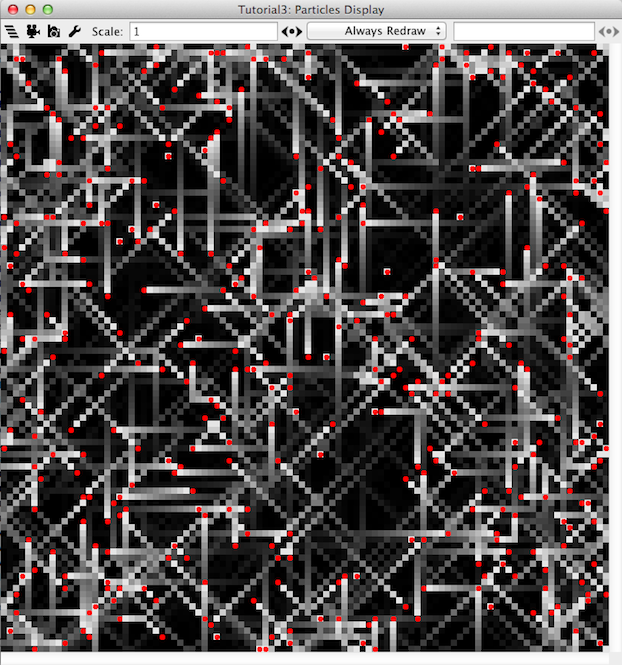
\includegraphics[width=0.4\textwidth]{part.png}
		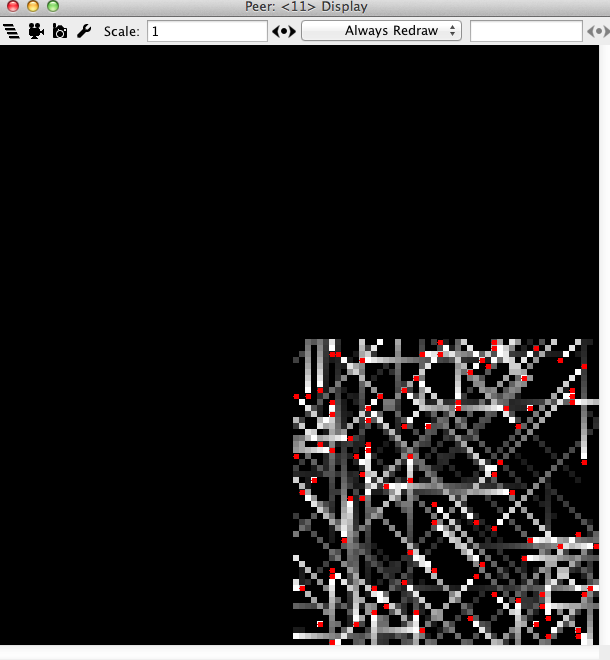
\includegraphics[width=0.2\textwidth]{ppp.png}
		\caption{Respectively \textit{Particles} and a \textit{DParticles}' parted field}
	\label{fig:dp01}
\end{figure}
\end{frame}
\end{document}
